\chapter{Results}\label{chap:Results}

% Update?
In this chapter, the results of the analysis are presented. \textbf{Chapter \ref{sec:Exploratory_Data_Analysis}} provides an overview of the data and explores the fairness of the dataset. 
\textbf{Chapter \ref{sec:Results}} presents the results of the analysis. \textbf{Chapter \ref{sec:Limitations}} discusses the limitations of the analysis.

\section{Exploratory Data Analysis}\label{sec:Exploratory_Data_Analysis}



\subsection{Data Overview}\label{subsec:Data_Overview}

The processed dataset contains two \textit{numerical} features: \textbf{interest\_rate} and \textbf{loan\_to\_value\_ratio}.
Their distributions can be seen in \textbf{Figure \ref{fig:CHXX_Numerical_Distributions_1}} and \textbf{Figure \ref{fig:CHXX_Numerical_Distributions_2}}.

\begin{figure}[h]
    \centering
    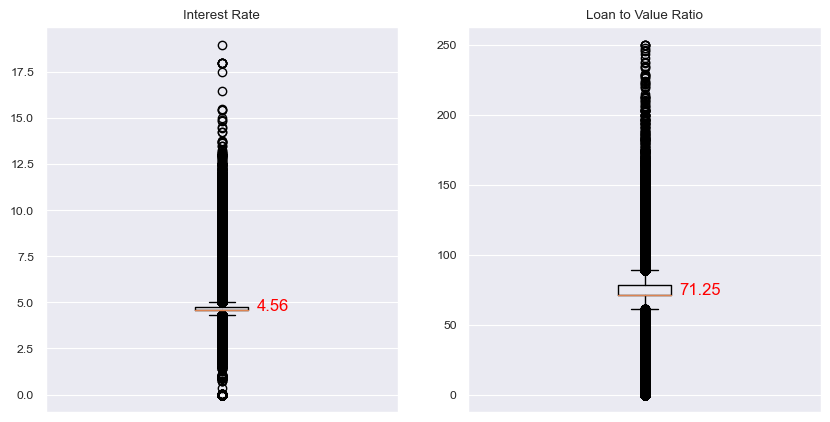
\includegraphics[width=0.85\textwidth]{CHXX_Numerical_Distributions_1.png}
    \caption{Boxplots of the Numerical Features}
    \label{fig:CHXX_Numerical_Distributions_1}
\end{figure}

\begin{figure}[h]
    \centering
    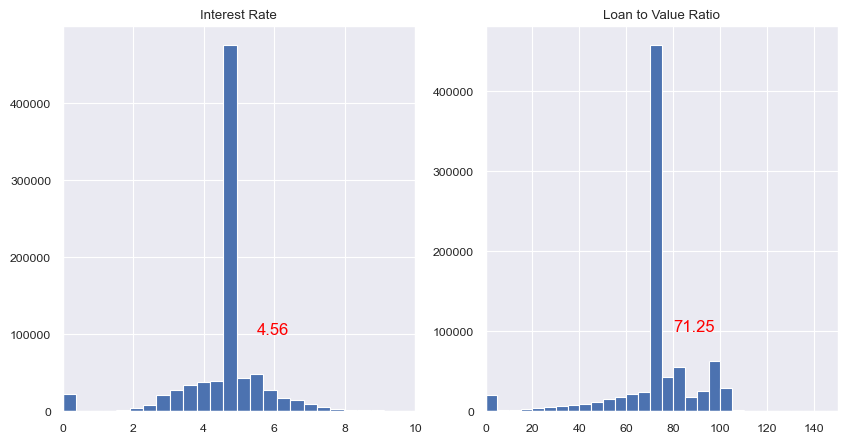
\includegraphics[width=0.85\textwidth]{CHXX_Numerical_Distributions_2.png}
    \caption{Histograms of the Numerical Features}
    \label{fig:CHXX_Numerical_Distributions_2}
\end{figure}

The results of the KNNImputer applying mean (annotated in red) values for all missing values show clearly here.

% Add analysis of categorical features

% Correlation Analysis?

\subsection{Fairness}\label{subsec:Fairness}

% Probably rename - tie to Hypothesis and Research Questions

% Graph on grant by race, accompanied by additional information from NN notebook like difference in groups etc.

Potential unfairness in the underlying data can be identified from assessing the distribution of the target variable across different groups.
\textbf{Figure \ref{fig:CHXX_Loan_Grant_By_Protected_Attribute}} shows the amount of (not) granted loans per race and by sex, the probabilities of being granted a loan across these groups can be found in \textbf{Table \ref{tab:loan_granting}}.\@

\begin{figure}[h]
    \centering
    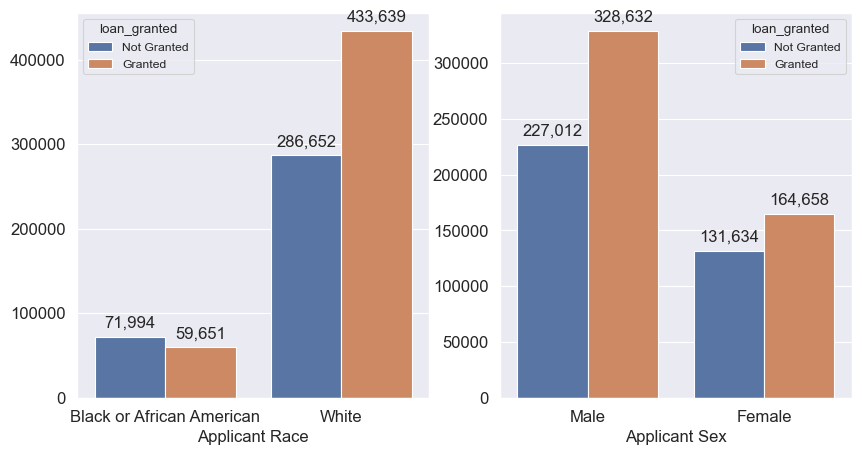
\includegraphics[width=0.85\textwidth]{CHXX_Loan_Grant_By_Protected_Attribute.png}
    \caption{Loan Grant by Protected Attribute}
    \label{fig:CHXX_Loan_Grant_By_Protected_Attribute}
\end{figure}

\begin{table}[htbp]
    \centering
      \begin{tabular}{lcc}
      \toprule
      \textbf{Applicant Race} & \textbf{Applicant Sex} & \textbf{Loan Granted (\%)} \\
      \midrule
      Black or African American & Male    & 46.4 \\
            & Female  & 44.1 \\
      White & Male    & 60.9 \\
            & Female  & 58.8 \\
      \bottomrule
      \end{tabular}%
      \caption{Loan Granting Statistics by Applicant Race and Sex}
    \label{tab:loan_granting}%
\end{table}%

Even though the focus of the analysis is on the \textit{applicant\_race-1} attribute, \textit{applicant\_sex} has been included as a second discriminating factor, as it also constitutes a protected attribute.
Inspection of the results depicted here does however imply that the issue of racial equality is more pronounced than that of inequality between the sexes.
A chi-squared test of independence proves that assumption of underlying inequality between races in the data, as the p-value is \textit{<0.01} and therefore H0 (equality in granted loans) can be rejected at any significance level.
Utilizing the aforementioned \textbf{AIF360} package to assess the mean difference of granted loans between the races in the underlying data amounts to a \textit{14.9\%} difference.

\section{Results}\label{sec:Results}        



\section{Limitations}\label{sec:Limitations}